\documentclass[ preprint, numerical, superscriptaddress, showkeys,
                svgnames, amssymb, aps, prb ]{revtex4-2}
\usepackage{graphicx, subcaption, array, booktabs, mathtools, extarrows,
            tikz, mhchem, physics2, fixdif, bm, derivative, lmodern, dsfont,
            CJKutf8, url, paracol}
\usetikzlibrary{arrows.meta}
\tikzset{> = Stealth}
\DeclareRobustCommand \iu {\mathrm i\mkern1mu}
\DeclareMathOperator \upe {e}
\usepackage[mono = false]{libertine}
\usephysicsmodule{ab, ab.braket, qtext.legacy, op.legacy, xmat}
\usepackage[final, nopatch = footnote]{microtype}
\usepackage{etoolbox, zref-clever, zref-titleref}
\zcsetup{cap, abbrev}
\makeatletter
\patchcmd{\frontmatter@abstract@produce}
  {\vskip200\p@\@plus1fil
   \penalty-200\relax
   \vskip-200\p@\@plus-1fil}{}{}{}
\makeatother
\counterwithin{equation}{section}
\renewcommand *\theequation{\arabic{section}.\arabic{equation}}
\graphicspath{{./media/}}

\begin{document}

\title{Band Structure of 2D Kagome Lattice: Tight-Binding
  Analysis with Nearest and Next-Nearest Neighbor Hopping}
\author{Mingyu Xia (夏明宇)}
\affiliation{Department of Physics, Westlake University}
\email{\ttfamily xiamingyu@westlake.edu.cn}
\date{2026-01-08 --- Final Project}

\begin{abstract}
  This article studies the Kagome lattice's electronic structure using a
  tight-binding approach. Deriving the dispersion relation for nearest-neighbor
  hopping reveals two dispersive bands and one flat band, which has been
  visualized through 3D/2D plots. Additionally, this article analyzes the band
  next-nearest-neighbor hopping, discussing how additional terms modify the
  band structure.
  \keywords{Kagome lattice, Tight-binding model, Dispersion relation,
    Geometric frustration, Second quantization}
\end{abstract}

\begin{CJK*}{UTF8}{gbsn}
\maketitle
\end{CJK*}

\section{Introduction}

\subsection{Background}

The kagome lattice was coined by Japanese physicist Kôdi Husimi, and first
appeared in a 1951 paper by his assistant Ichirō Shōji~\cite{WikipediA}.
It has emerged as a paradigmatic platform for studying
geometric frustration due to its unique combination of cornersharing triangles.
This geometric arrangement naturally leads to competing interactions and
degenerate ground states, making it an ideal system for investigating exotic
quantum phases such as quantum spin liquids, which evade conventional magnetic
ordering even at absolute zero temperature.

The lattice's inherent frustration arises from the impossibility of
simultaneously minimizing all pairwise interactions in antiferromagnetically
coupled Ising spins on triangular units.

Recent years have witnessed renewed interest in Kagome materials driven by
experimental discoveries of real materials with Kagome-like structures, such as
Herbertsmithite (\ce{ZnCu3(OH)6Cl2}), which exhibits signatures of quantum spin
liquid behavior, and \ce{AV3Sb5} (A = K, Rb, Cs) compounds that display
unconventional superconductivity and charge density wave orders.

\subsection{Lattice Structure}

Different from the two types of sites in honeycomb lattice, the Kagome lattice
has 3 types of sites, \textcolor{blue}{$A$ (blue)}, \textcolor{red}{$B$ (red)},
and \textcolor{Green}{$C$ (green)}, respectively.

\begin{figure}[htbp]
  \begin{minipage}[t]{.48\linewidth}
    \centering
    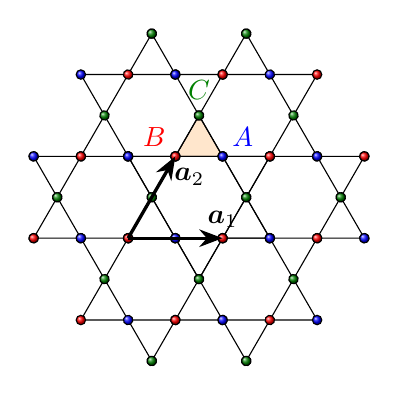
\begin{tikzpicture}[scale = .6]
      \fill [orange, opacity = .2]
        (.5,{sqrt(3)}) node [opacity = 1, blue, above right] {$A$} --++
        (-1,0) node [opacity = 1, red, above left] {$B$} --++
        (60:1) node [opacity = 1, Green, above = .5ex] {$C$} -- cycle;
      \foreach \i in {0, 180}
        {
      \begin{scope}[rotate around = {\i:(0,{sqrt(3)/2})}]
        \draw (-3.5,0) --++ (5,0) --++ (120:5) --++ (240:5) -- cycle;
        \draw (-1.5,0) --++ (5,0) --++ (120:5) --++ (240:5) -- cycle;
        \draw (-2.5,{-sqrt(3)}) --++ (5,0) --++ (120:5) --++ (240:5) -- cycle;
      \end{scope}
        }
      \foreach \i in {0, 180}
        {
      \begin{scope}[rotate around = {\i:(0,{sqrt(3)/2})}]
        \foreach \j in {0, 2}
        {
      \begin{scope}[xshift = \j cm]
        \shade [draw, ball color = blue] (-2.5,0) circle (.1);
        \shade [draw, ball color = blue] (-.5,0) circle (.1);
        \shade [draw, ball color = blue] (1.5,0) circle (.1);
        \shade [draw, ball color = red] (-3.5,0) circle (.1);
        \shade [draw, ball color = red] (-1.5,0) circle (.1);
        \shade [draw, ball color = red] (.5,0) circle (.1);
        \begin{scope}[rotate around = {60:(-3.5,0)}]
          \shade [draw, ball color = red] (-3.5,0) circle (.1);
          \shade [draw, ball color = red] (-1.5,0) circle (.1);
          \shade [draw, ball color = red] (.5,0) circle (.1);
          \shade [draw, ball color = Green] (-2.5,0) circle (.1);
          \shade [draw, ball color = Green] (-.5,0) circle (.1);
          \shade [draw, ball color = Green] (1.5,0) circle (.1);
        \end{scope}
        \begin{scope}[rotate around = {-60:(1.5,0)}]
          \shade [draw, ball color = Green] (-3.5,0) circle (.1);
          \shade [draw, ball color = Green] (-1.5,0) circle (.1);
          \shade [draw, ball color = Green] (.5,0) circle (.1);
          \shade [draw, ball color = blue] (-2.5,0) circle (.1);
          \shade [draw, ball color = blue] (-.5,0) circle (.1);
          \shade [draw, ball color = blue] (1.5,0) circle (.1);
        \end{scope}
        \shade [draw, ball color = red] (-2.5,{-sqrt(3)}) circle (.1);
        \shade [draw, ball color = blue] (.5,{-sqrt(3)}) circle (.1);
      \end{scope}
        }
      \end{scope}
        }
      \draw [very thick, ->] (-1.5,0) --++ (2,0)
       node [above] {$\bm a_1$};
      \draw [very thick, ->] (-1.5,0) --++ (60:2)
       node [near end, right] {$\bm a_2$};
    \end{tikzpicture}
  \end{minipage}
  \hfill
  \begin{minipage}[t]{.48\linewidth}
    \centering
    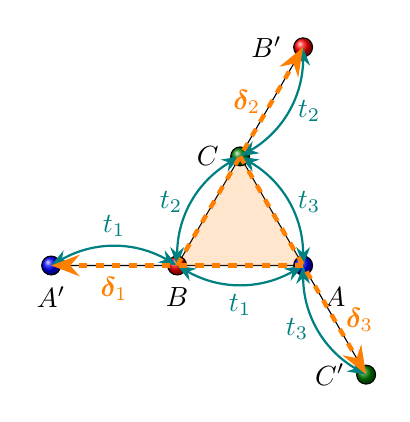
\begin{tikzpicture}[scale = .8]
      \draw (2,0) -- (-2,0)
            (0,0) -- (2,{2*sqrt(3)})
            (1,{sqrt(3)}) -- (3,{-sqrt(3)});
      \fill [orange, opacity = .2] (0,0) -- (1,{sqrt(3)}) -- (2,0) -- cycle;
      \shade [draw, ball color = blue] (2,0) circle (.15) coordinate (A)
       node [below right = .15cm] {$A$};
      \shade [draw, ball color = red] (0,0) circle (.15) coordinate (B)
       node [below = .15cm] {$B$};
      \shade [draw, ball color = Green] (1,{sqrt(3)}) circle (.15)
       coordinate (C) node [left = .15cm] {$C$};

      \shade [draw, ball color = blue] (-2,0) circle (.15)
       coordinate (A') node [below = .15cm] {$A'$};
      \shade [draw, ball color = red] (2,{2*sqrt(3)}) circle (.15)
       coordinate (B') node [left = .15cm] {$B'$};
      \shade [draw, ball color = Green] (3,{-sqrt(3)}) circle (.15)
       coordinate (C') node [left = .15cm] {$C'$};
      \draw [thick, <->, teal] (A) to[bend left] node [below] {$t_1$} (B);
      \draw [thick, <->, teal] (B) to[bend left] node [left] {$t_2$} (C);
      \draw [thick, <->, teal] (C) to[bend left] node [right] {$t_3$} (A);
      \draw [thick, <->, teal] (B) to[bend right] node [above] {$t_1$} (A');
      \draw [thick, <->, teal] (C) to[bend right] node [right] {$t_2$} (B');
      \draw [thick, <->, teal] (A) to[bend right] node [left] {$t_3$} (C');
      \draw [ultra thick, dashed, ->, orange] (B) --
       node [left, near end] {$\bm \delta_2$} (B');
      \draw [ultra thick, dashed, ->, orange] (A) --
       node [below, near end] {$\bm \delta_1$} (A');
      \draw [ultra thick, dashed, ->, orange] (C) --
       node [right, near end] {$\bm \delta_3$} (C');
    \end{tikzpicture}
  \end{minipage}
  \caption{Top view of the Kagome Lattice and
    tight-binding model with NN hopping}
  \zlabel{fig:Kagome}
\end{figure}

The three sites in the unit cell form a regular triangle, which is shaded
in~\zcref{fig:Kagome}. The primitive vectors and reciprocal (Honeycomb, not
shown in the article) vectors are
\begin{equation}
  \bm a_1 = a(2,0), \quad \bm a_2 = a(1, \sqrt3); \quad
  \bm b_1 = \frac{2\pi}{a}\ab(0, \frac1{\sqrt3}), \quad
  \bm b_2 = \frac{2\pi}{a}\ab(\frac12, -\frac1{2\sqrt3}).
\end{equation}
Simply taking the unit cell located at $\bm r$. Then, each site in the
unit cell has 2 NN hoppings, pointing out by the lattice vectors
\begin{equation}
  \bm \delta_1 = a(-2,0),     \quad
  \bm \delta_2 = a(1, \sqrt3),\quad
  \bm \delta_3 = a(1,-\sqrt3),
  \label{eq:vectors}
\end{equation}
where $a$ is the lattice constant, the distance between any two NN lattices.

\section{Model Hamiltonian}

In this model, consider the nearest-neighbor (NN) hopping with different
hopping magnitude $t_1$, $t_2$, and $t_3$.
The Hamiltonian illustrates the tight-binding model in terms of second
quantization~\cite{PhysRevB.102.045151}
\begin{equation}
  \mathcal H = -\sum_{\bm r}[
    t_1(\hat a_{\bm r}^\dagger \hat b_{\bm r}
      + \hat b_{\bm r}^\dagger \hat a_{\bm r+\bm\delta_1})
  + t_2(\hat b_{\bm r}^\dagger \hat c_{\bm r}
      + \hat c_{\bm r}^\dagger \hat b_{\bm r+\bm\delta_2})
  + t_3(\hat c_{\bm r}^\dagger \hat a_{\bm r}
      + \hat a_{\bm r}^\dagger \hat c_{\bm r+\bm\delta_3})]
  + \text{H.c.}
  \label{eq:Hamiltonian_NN}
\end{equation}
Assume there are $N$ $A$-, $B$-, and $C$- type sites in total.
Applying the Fourier transformation to the Fermion operators
\begin{alignat*}{3}
  & \hat a_{\bm r}
  = \frac1{\sqrt N} \sum_{\bm k} \upe^{\iu \bm k\cdot \bm r} \hat a_{\bm k},
  &\hspace*{2\arraycolsep}
  & \hat b_{\bm r}
  = \frac1{\sqrt N} \sum_{\bm k} \upe^{\iu \bm k\cdot \bm r} \hat b_{\bm k},
  &\hspace*{2\arraycolsep}
  & \hat c_{\bm r}
  = \frac1{\sqrt N} \sum_{\bm k} \upe^{\iu \bm k\cdot \bm r} \hat c_{\bm k},\\
  & \hat a_{\bm r+\bm\delta_1}
  = \frac1{\sqrt N} \sum_{\bm k}
    \upe^{\iu \bm k\cdot (\bm r + \bm \delta_1)} \hat a_{\bm k},
& & \hat b_{\bm r+\bm\delta_2}
  = \frac1{\sqrt N} \sum_{\bm k}
    \upe^{\iu \bm k\cdot (\bm r + \bm \delta_2)} \hat b_{\bm k},
& & \hat c_{\bm r+\bm\delta_3}
  = \frac1{\sqrt N} \sum_{\bm k}
    \upe^{\iu \bm k\cdot (\bm r + \bm \delta_3)} \hat c_{\bm k}.
\shortintertext{Similar for their Hermite conjugates}
  & \hat a_{\bm r}^\dagger
  = \frac1{\sqrt N} \sum_{\bm k}
    \upe^{-\iu \bm k\cdot \bm r} \hat a_{\bm k}^\dagger,
& & \hat b_{\bm r}^\dagger
  = \frac1{\sqrt N} \sum_{\bm k}
    \upe^{-\iu \bm k\cdot \bm r} \hat b_{\bm k}^\dagger,
& & \hat c_{\bm r}^\dagger
  = \frac1{\sqrt N} \sum_{\bm k}
    \upe^{-\iu \bm k\cdot \bm r} \hat c_{\bm k}^\dagger,\\
  & \hat a_{\bm r+\bm\delta_1}^\dagger
  = \frac1{\sqrt N} \sum_{\bm k}
    \upe^{-\iu \bm k\cdot (\bm r + \bm \delta_1)} \hat a_{\bm k}^\dagger,
& & \hat b_{\bm r+\bm\delta_2}^\dagger
  = \frac1{\sqrt N} \sum_{\bm k}
    \upe^{-\iu \bm k\cdot (\bm r + \bm \delta_2)} \hat b_{\bm k}^\dagger,
& & \hat c_{\bm r+\bm\delta_3}^\dagger
  = \frac1{\sqrt N} \sum_{\bm k}
    \upe^{-\iu \bm k\cdot (\bm r + \bm \delta_3)} \hat c_{\bm k}^\dagger.
\end{alignat*}
Substituting the transformed operators into the
Hamiltonian~\eqref{eq:Hamiltonian_NN}
\begin{multline*}
  \mathcal H = -\sum_{\bm k} [
    t_1(1 + \upe^{-\iu \bm k\cdot\bm\delta_1})
    \hat a_{\bm k}^\dagger \hat b_{\bm k}
  + t_2(1 + \upe^{-\iu \bm k\cdot\bm\delta_2})
    \hat b_{\bm k}^\dagger \hat c_{\bm k}
  + t_3(1 + \upe^{-\iu \bm k\cdot\bm\delta_3})
    \hat c_{\bm k}^\dagger \hat a_{\bm k}]
  + \text{H.c.}\\
= -\sum_{\bm k}[\tilde t_1 \hat a_{\bm k}^\dagger \hat b_{\bm k}
              + \tilde t_2 \hat b_{\bm k}^\dagger \hat c_{\bm k}
              + \tilde t_3 \hat c_{\bm k}^\dagger \hat a_{\bm k}]
  + \text{H.c.}
\end{multline*}
Here $\tilde t_i$ are used for simplification, and the identity
\[
  \sum_{A,B,C} \upe^{\iu(\bm k' - \bm k)\cdot\bm r} = N\delta_{\bm k',\bm k}
\]
is applied.
\section{Dispersion Relation}

Diagonalizing the Hamiltonian first. The Hamiltonian can be written as
\begin{equation}
  \mathcal H = \sum_{\bm k} \Psi_{\bm k}^\dagger \tilde{\mathcal H} \Psi_{\bm k}
= \sum_{\bm k}
  \begin{pmatrix}
    \hat a_{\bm k}^\dagger & \hat b_{\bm k}^\dagger & \hat c_{\bm k}^\dagger
  \end{pmatrix}
  \begin{pmatrix}
    0 & -\tilde t_1 & -\tilde t_3^*\\
    -\tilde t_1^* & 0 & -\tilde t_2\\
    -\tilde t_3 & -\tilde t_2^* & 0
  \end{pmatrix}
  \begin{pmatrix}
    \hat a_{\bm k}\\ \hat b_{\bm k}\\ \hat c_{\bm k}
  \end{pmatrix},
  \label{eq:diagonalized_Hamiltonian}
\end{equation}
it is naturally that all diagonal elements of $\tilde{\mathcal H}$ are zero
since there is not exist the elements
like $\hat a_{\bm k}^\dagger \hat a_{\bm k}$ in the transformed Hamiltonian.
The diagonalized Hamiltonian~\eqref{eq:diagonalized_Hamiltonian} can be
determined by comparing
\[
  \mathcal H =
  \sum_{\bm k}
  \begin{pmatrix}
    \hat a_{\bm k}^\dagger & \hat b_{\bm k}^\dagger & \hat c_{\bm k}^\dagger
  \end{pmatrix}
  \pxmat{-H}{3}{3}
  \begin{pmatrix}
    \hat a_{\bm k}\\ \hat b_{\bm k}\\ \hat c_{\bm k}
  \end{pmatrix}
\]
with the transformed Hamiltonian.

From the eigenequation $\det(\tilde{\mathcal H} - E\mathds 1) = 0$, one
can obtain a cubic polynomial in $E$
\begin{equation}
  E^3 - E(|\tilde t_1|^2 + |\tilde t_2|^2 + |\tilde t_3|^2)
      + \tilde t_1 \tilde t_2 \tilde t_3
      + \tilde t_1^* \tilde t_2^* \tilde t_3^* = 0.
  \label{eq:dispersion_relation}
\end{equation}
Expanding $|\tilde t_1|^2$
\begin{align*}
  |\tilde t_1|^2 & = \tilde t_1\tilde t_1^*
= t_1^2(1 + \upe^{-\iu\bm k\cdot\bm\delta_1})
       (1 + \upe^{+\iu\bm k\cdot\bm\delta_1})
= t_1^2[2 + 2\cos(\bm k\cdot\bm\delta_1)].
  \shortintertext{Similarly for $|\tilde t_2|^2$ and $|\tilde t_3|^2$}
  |\tilde t_2|^2 & = t_2^2[2 + 2\cos(\bm k\cdot\bm\delta_2)],\quad
  |\tilde t_3|^2   = t_3^2[2 + 2\cos(\bm k\cdot\bm\delta_3)].
\end{align*}
Expanding $\tilde t_1 \tilde t_2 \tilde t_3$
\begin{align*}
& \begin{multlined}[t][.85\linewidth]
  \tilde t_1 \tilde t_2 \tilde t_3 = t_1 t_2 t_3[1
+ \upe^{-\iu\bm k\cdot\bm\delta_1}
+ \upe^{-\iu\bm k\cdot\bm\delta_2}
+ \upe^{-\iu\bm k\cdot\bm\delta_3}\\
+ \upe^{-\iu\bm k\cdot(\bm\delta_2+\bm\delta_3)}
+ \upe^{-\iu\bm k\cdot(\bm\delta_1+\bm\delta_3)}
+ \upe^{-\iu\bm k\cdot(\bm\delta_1+\bm\delta_2)}
+ \upe^{-\iu\bm k\cdot(\bm\delta_1+\bm\delta_2+\bm\delta_3)}].
\end{multlined}\\
\shortintertext{Similarly for the conjugate}
& \begin{multlined}[t][.85\linewidth]
  \tilde t_1^* \tilde t_2^* \tilde t_3^* = t_1 t_2 t_3[1
+ \upe^{+\iu\bm k\cdot\bm\delta_1}
+ \upe^{+\iu\bm k\cdot\bm\delta_2}
+ \upe^{+\iu\bm k\cdot\bm\delta_3}\\
+ \upe^{+\iu\bm k\cdot(\bm\delta_2+\bm\delta_3)}
+ \upe^{+\iu\bm k\cdot(\bm\delta_1+\bm\delta_3)}
+ \upe^{+\iu\bm k\cdot(\bm\delta_1+\bm\delta_2)}
+ \upe^{+\iu\bm k\cdot(\bm\delta_1+\bm\delta_2+\bm\delta_3)}].
\end{multlined}
\end{align*}
Combining the two terms
\begin{align*}
  \tilde t_1 \tilde t_2 \tilde t_3 + \tilde t_1^* \tilde t_2^* \tilde t_3^*
& = t_1 t_2 t_3[2 + 2\cos(\bm k \cdot \bm\delta_1)
    + 2\cos(\bm k \cdot \bm\delta_2)
    + 2\cos(\bm k \cdot \bm\delta_3)\\
& \quad
    + 2\cos(\bm k \cdot (\bm\delta_2 + \bm\delta_3))
    + 2\cos(\bm k \cdot (\bm\delta_1 + \bm\delta_3))
    + 2\cos(\bm k \cdot (\bm\delta_1 + \bm\delta_2))\\
& \quad
    + 2\cos(\bm k \cdot (\bm\delta_1 + \bm\delta_2 + \bm\delta_3))]\\
& = 4t_1 t_2 t_3[1 + \cos(\bm k \cdot \bm\delta_1)
    + \cos(\bm k \cdot \bm\delta_2) + \cos(\bm k \cdot \bm\delta_3)],
\end{align*}
where $\bm\delta_i + \bm\delta_j = -\epsilon_{ijk}\bm\delta_k$,
$\sum_i \bm\delta_i = 0$ is used from~\eqref{eq:vectors}.

Then, substituting these terms into the dispersion
relation~\eqref{eq:dispersion_relation}
\begin{equation}
  E^3 - 2E \sum_i^3 t_i^2 (1 + \cos(\bm k \cdot \bm\delta_i))
      + 4t_1t_2t_3 \ab[1 + \sum_i^3 \cos(\bm k \cdot \bm\delta_i)] = 0.
  \label{eq:dispersion_relation_expand}
\end{equation}
This is a universal result.

\section{Result Discussion}

Simply taking $t_1 = t_2 = t_3 = t$, then the dispersion
relation~\eqref{eq:dispersion_relation_expand} becomes
\begin{equation}
  E^3 - 2Et^2\ab[3 + \sum_i^3 \cos(\bm k \cdot \bm\delta_i)]
      + 4t^3 \ab[1 + \sum_i^3 \cos(\bm k \cdot \bm\delta_i)] = 0.
  \label{eq:dispersion_eqt}
\end{equation}
By using the solution of the cubic equation, there are three
solutions for~\eqref{eq:dispersion_eqt}
\begin{subequations}
\begin{align}
  E_+           &
= t\ab[-1 + \sqrt{\textstyle 3 + 2\sum_i^3 \cos(\bm k \cdot \bm\delta_i)}],
  \label{eq:band_positive}\\
  E_-           &
= t\ab[-1 - \sqrt{\textstyle 3 + 2\sum_i^3 \cos(\bm k \cdot \bm\delta_i)}],
  \label{eq:band_negative}\\
  E_\text{flat} & = 2t,\label{eq:band_flat}
\end{align}
\end{subequations}
i.e., two dispersive bands~\eqref{eq:band_positive}
and~\eqref{eq:band_negative}, and one flat band~\eqref{eq:band_flat}.

\subsection{Band Structure}

\textsf{Python} is used to plot its band structure.
The hopping magnitude $t$ is taken as $1$. \zcref{fig:3Dband} shows the energy
band structure for the two dispersive bands and the one flat band.

\begin{figure}[htbp]
  \begin{minipage}{.48\linewidth}
    \centering
    \includegraphics[page = 1, width = \linewidth]{kagome_bands.pdf}
  \end{minipage}
  \hfill
  \begin{minipage}{.48\linewidth}
    \centering
    \includegraphics[page = 2, width = \linewidth]{kagome_bands.pdf}
  \end{minipage}
  \caption{3D band structure for NN hopping under different perspectives}
  \zlabel{fig:3Dband}
\end{figure}

In momentum space, \zcref{fig:2Dband} demonstrates the contours for the two
dispersive bands in the $k_x$-$k_y$ plane.

\begin{figure}[htbp]
  \begin{minipage}{.48\linewidth}
    \centering
    \includegraphics[page = 3, width = \linewidth]{kagome_bands.pdf}
  \end{minipage}
  \hfill
  \begin{minipage}{.48\linewidth}
    \centering
    \includegraphics[page = 4, width = \linewidth]{kagome_bands.pdf}
  \end{minipage}
  \caption{2D band structure for the two dispersive bands}
  \zlabel{fig:2Dband}
\end{figure}

\subsection{Properties around the Dirac Point}

Taking the simplest $K$-point: $\frac{2\pi}{a}\ab(0, \frac1{\sqrt3})$.
At this point, this dispersion relation becomes
\[
  E_+ = t[-1 \pm \sqrt{3 + 2(\cos(0) + \cos(2\pi) + \cos(-2\pi))}]
      = 2t = E_\text{flat},\quad E_- = -4t,
\]
which is implied in~\zcref{fig:3Dband}: $E_\text{flat}$ and $E_+$ are tangent
at four $K$-points.

Sightly taking $\bm k = \bm b_2 + \bm q$ with $|\bm q| \ll 1$, then, the
dispersion relation becomes
\[
  E_+ = t[-1 + \sqrt{3 + 2(3 - 12\pi^2|\bm q|^2)}]
= t\ab(2 - \frac43\pi^2|\bm q^2|),\quad
  E_- = t\ab(-4 + \frac43\pi^2|\bm q|^2),
\]
which indicates that the dispersive bands around the Dirac points are parabolic.

\section{Advanced Study: The Next-Nearest Neighbor Hopping Term}

Assume the hopping magnitude between the NNN $t_i'$, just add the NNN hopping
in the right part of~\zcref{fig:Kagome} is enough, since all the NNN and NN
hopping can be covered by simply splicing each unit, as shown
in~\zcref{fig:NNN_splice}
\setbox0=\hbox{
  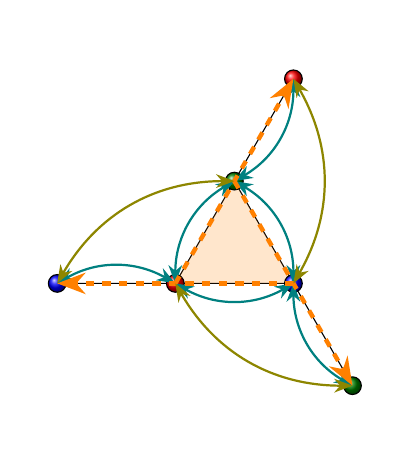
\begin{tikzpicture}[scale = .75]
    \path (-2.5,{2.5*sqrt(3)}) rectangle (3.5,{-1.5*sqrt(3)});
    \draw (2,0) -- (-2,0)
          (0,0) -- (2,{2*sqrt(3)})
          (1,{sqrt(3)}) -- (3,{-sqrt(3)});
    \fill [orange, opacity = .2] (0,0) -- (1,{sqrt(3)}) -- (2,0) -- cycle;
    \shade [draw, ball color = blue] (2,0) circle (.15) coordinate (A);
    \shade [draw, ball color = red] (0,0) circle (.15) coordinate (B);
    \shade [draw, ball color = Green] (1,{sqrt(3)}) circle (.15)
     coordinate (C);
    \shade [draw, ball color = blue] (-2,0) circle (.15)
     coordinate (A');
    \shade [draw, ball color = red] (2,{2*sqrt(3)}) circle (.15)
     coordinate (B');
    \shade [draw, ball color = Green] (3,{-sqrt(3)}) circle (.15)
     coordinate (C');
    \draw [thick, <->, teal] (A) to[bend left]  (B);
    \draw [thick, <->, teal] (B) to[bend left]  (C);
    \draw [thick, <->, teal] (C) to[bend left]  (A);
    \draw [thick, <->, teal] (B) to[bend right] (A');
    \draw [thick, <->, teal] (C) to[bend right] (B');
    \draw [thick, <->, teal] (A) to[bend right] (C');
    \draw [ultra thick, dashed, ->, orange] (B) -- (B');
    \draw [ultra thick, dashed, ->, orange] (A) -- (A');
    \draw [ultra thick, dashed, ->, orange] (C) -- (C');
    \draw [thick, <->, olive] (A) to[bend right] (B');
    \draw [thick, <->, olive] (B) to[bend right] (C');
    \draw [thick, <->, olive] (C) to[bend right] (A');
  \end{tikzpicture}
}
\begin{figure}[htbp]
  \[
    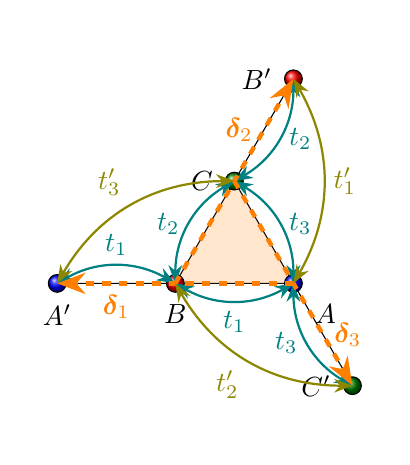
\begin{tikzpicture}[baseline, scale = .75]
      \path (-2.5,{2.5*sqrt(3)}) rectangle (3.5,{-1.5*sqrt(3)});
      \draw (2,0) -- (-2,0)
            (0,0) -- (2,{2*sqrt(3)})
            (1,{sqrt(3)}) -- (3,{-sqrt(3)});
      \fill [orange, opacity = .2] (0,0) -- (1,{sqrt(3)}) -- (2,0) -- cycle;
      \shade [draw, ball color = blue] (2,0) circle (.15) coordinate (A)
       node [below right = .15cm] {$A$};
      \shade [draw, ball color = red] (0,0) circle (.15) coordinate (B)
       node [below = .15cm] {$B$};
      \shade [draw, ball color = Green] (1,{sqrt(3)}) circle (.15)
       coordinate (C) node [left = .15cm] {$C$};
      \shade [draw, ball color = blue] (-2,0) circle (.15)
       coordinate (A') node [below = .15cm] {$A'$};
      \shade [draw, ball color = red] (2,{2*sqrt(3)}) circle (.15)
       coordinate (B') node [left = .15cm] {$B'$};
      \shade [draw, ball color = Green] (3,{-sqrt(3)}) circle (.15)
       coordinate (C') node [left = .15cm] {$C'$};
      \draw [thick, <->, teal] (A) to[bend left] node [below] {$t_1$} (B);
      \draw [thick, <->, teal] (B) to[bend left] node [left] {$t_2$} (C);
      \draw [thick, <->, teal] (C) to[bend left] node [right] {$t_3$} (A);
      \draw [thick, <->, teal] (B) to[bend right] node [above] {$t_1$} (A');
      \draw [thick, <->, teal] (C) to[bend right] node [right] {$t_2$} (B');
      \draw [thick, <->, teal] (A) to[bend right] node [left] {$t_3$} (C');
      \draw [ultra thick, dashed, ->, orange] (B) --
       node [left, near end] {$\bm \delta_2$} (B');
      \draw [ultra thick, dashed, ->, orange] (A) --
       node [below, near end] {$\bm \delta_1$} (A');
      \draw [ultra thick, dashed, ->, orange] (C) --
       node [right, near end] {$\bm \delta_3$} (C');
      \draw [thick, <->, olive] (A) to[bend right]
       node [right] {$t_1'$} (B');
      \draw [thick, <->, olive] (B) to[bend right]
       node [below left] {$t_2'$} (C');
      \draw [thick, <->, olive] (C) to[bend right]
       node [above left] {$t_3'$} (A');
    \end{tikzpicture}
    \quad \longrightarrow \qquad
    \begin{tikzpicture}[baseline, scale = 1.2]
      \node [inner sep = 0pt, scale = .6] at (0,0) {\usebox0};
      \node [inner sep = 0pt, scale = .6] at (1.5,0) {\usebox0};
      \node [inner sep = 0pt, scale = .6] at (-1.5,0) {\usebox0};
      \node [inner sep = 0pt, scale = .6] at (.75,{.75*sqrt(3)}) {\usebox0};
      \node [inner sep = 0pt, scale = .6] at (-.75,{.75*sqrt(3)}) {\usebox0};
      \node [inner sep = 0pt, scale = .6] at (2.25,{.75*sqrt(3)}) {\usebox0};
      \node [inner sep = 0pt, scale = .6] at (3,0) {\usebox0};
    \end{tikzpicture}
  \]
  \caption{TB model with NN and NNN hopping}
  \zlabel{fig:NNN_splice}
\end{figure}

The total Hamiltonian can be separated into two terms: The NN
(Nearest neighbor) one and the NNN (Next-Nearest Neighbor) one
\begin{equation}
  \mathcal H' = \mathcal H_\text{NN} + \mathcal H_\text{NNN}.
\end{equation}
The NN term has already given in~\eqref{eq:Hamiltonian_NN},
similarly, the NNN term can be expressed as~\cite{PhysRevB.80.113102}
\begin{equation}
\begin{aligned}
  \mathcal H_\text{NNN} & = -\sum_{\bm r}[t_1'(
    \hat a_{\bm r}^\dagger \hat b_{\bm r+\bm\delta_2}
  + \hat b_{\bm r}^\dagger \hat c_{\bm r+\bm\delta_3}
  + \hat c_{\bm r}^\dagger \hat a_{\bm r+\bm\delta_1})] + \text{H.c.}\\
& = \sum_{\bm k}
  \Psi_{\bm k}^\dagger
  \begin{psmallmatrix}
    0 & -t_1'\upe^{+\iu\bm k\cdot\bm\delta_2} &
        -t_3'\upe^{-\iu\bm k\cdot\bm\delta_1}\\
        -t_1'\upe^{-\iu\bm k\cdot\bm\delta_2} & 0 &
        -t_2'\upe^{+\iu\bm k\cdot\bm\delta_3}\\
        -t_3'\upe^{+\iu\bm k\cdot\bm\delta_1} &
        -t_2'\upe^{-\iu\bm k\cdot\bm\delta_3} & 0
  \end{psmallmatrix}
  \Psi_{\bm k}
= \sum_{\bm k}
  \Psi_{\bm k}^\dagger
  \begin{psmallmatrix}
    0 & -\tilde t_1' & -\tilde t_3'^*\\
    -\tilde t_1'^* & 0 & -\tilde t_2'\\
    -\tilde t_3' & -\tilde t_2'^* & 0
  \end{psmallmatrix}
  \Psi_{\bm k}.
\end{aligned}
\end{equation}
Similarly to the NN case, let $\det(\tilde{\mathcal H'} - E\mathds 1) = 0$,
we will obtain a very long equation of the dispersion relation.
For simplification, sightly taking $t_1' = t_2' = t_3' = t'$, then
\begin{equation}
  E^3 - 3E|t + t'|^2 + (\tilde t + \tilde t')^3
                     + (\tilde t^* + \tilde t'^*)^3 = 0,
\end{equation}
and the energy band can be plotted from this equation.

It is interesting that the diagonal of the transformed Hamiltonian is always
zero in the NN and NNN cases. So, if we further consider a farther NNN hopping
(actually, it is NNNN hopping) instead of the NNN hopping right now,
then taking the hopping magnitude between $A$ and
$A'$ is $t_1''$, $B$ and $B'$ is $t_2''$, $C$ and $C'$ is $t_3''$.
Finally, an extra term will be raised in the total Hamiltonian
\begin{equation}
  \mathcal H_\text{NNNN} = -\sum_{\bm r}[
    t_1'' \hat a_{\bm r}^\dagger \hat a_{\bm r+\bm\delta_1}
  + t_2'' \hat b_{\bm r}^\dagger \hat b_{\bm r+\bm\delta_2}
  + t_3'' \hat c_{\bm r}^\dagger \hat c_{\bm r+\bm\delta_3}] + \text{H.c.},
\end{equation}
and the Hamiltonian matrix in momentum space becomes
\begin{equation}
  \tilde{\mathcal H}' =
  \begin{pmatrix}
    -2t_1''\cos(\bm k \cdot \bm \delta_1) &
    -t_1(1 + \upe^{-\iu\bm k\cdot\bm\delta_1}) &
    -t_2(1 + \upe^{+\iu\bm k\cdot\bm\delta_2})\\
    -t_1(1 + \upe^{+\iu\bm k\cdot\bm\delta_1}) &
    -2t_2''\cos(\bm k \cdot \bm \delta_2) &
    -t_3(1 + \upe^{-\iu\bm k\cdot\bm\delta_3})\\
    -t_2(1 + \upe^{-\iu\bm k\cdot\bm\delta_2}) &
    -t_3(1 + \upe^{+\iu\bm k\cdot\bm\delta_3}) &
    -2t_3'' \cos(\bm k \cdot \bm \delta_3)
  \end{pmatrix}.
\end{equation}
One can obtain the dispersion relation
via $\det(\tilde{\mathcal H}' - E\mathds 1) = 0$.

\bibliography{reference}

\end{document}